\chapter{Background and Literature Review} \label{chap:sota}

\section*{}

This section will dive deep on previously done work related to this project. First, a Background is provided, for the reader to have context on some relevant work and information that precedes the findings present in the following sections. Second, since the goal is to develop a complete application, there will be an analysis on the specific problems, and how they have been solved in the literature. Then, there will be a comparison between a similar work and similar existing applications.

\section*{Background}

Since this project is intended for general use, the easiest and most common client available to users is the web client, also known as a web browser. In the early stages of the web, the applications followed a server-client architecture where the client had little to no work: it just rendered some previously compiled HTML and CSS on the page and the interaction with the server was made through HTML forms. Later on, JavaScript usage increased, and the pages started to be a bit more dynamic \cite{ShklarRosen09}. Still, it wasn't until more performant and portable devices such as the iPhone were available to the public, that web applications started to tilt their focus to the client side. More recently, we start to see "Single Page Applications", which harness the client-side JavaScript capabilities to simulate legacy web interactions such as changing to another page or view without actually reloading the page, trading client-side work for network load \cite{Lugo-Cordero2015} \cite{Derezinska2020} \cite{Mesbah2007} \cite{Mesbah2007a}. In this architecture, there still exists a server and clients (the web browsers), however, the server serves usually a REST API, and a bare-bones HTML document which serves as a base for the clients to render the rest of the document with JS, based on API calls results. There is also a mixed option, where the server handles some logic, usually related to session management or localization, and responds with an HTML document that already has some information to prevent the client-side to take too much time on work that will happen on every request. On the web, there are some frameworks that allow this more recent architecture such as React \cite{React}, Vue \cite{Vue} and Angular \cite{Angular}.

\begin{figure}[t]
    \begin{center}
      \leavevmode
      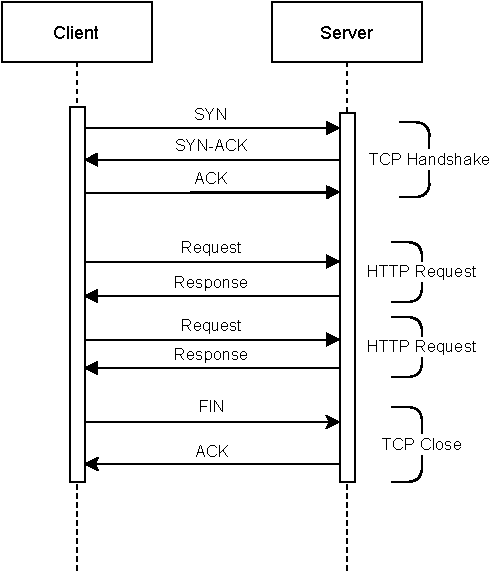
\includegraphics[width=0.6\textwidth]{http-protocol.pdf}
      \caption{HTTP protocol example interactions}
      \label{fig:http-protocol}
    \end{center}
  \end{figure}

Since the web uses the HTTP Protocol \cite{http1-1protocol} \cite{http2protocol}, it is quite hard to achieve some real-time behavior with good performance, due to the protocol's design \cite{Spero1994}. As can be seen in Fig. \ref{fig:http-protocol}, every data transfer starts with a request and ends with a response. It is therefore tied to this two-step process, which limits its potential. In order to allow a more performant way of data transmission between client and server, similar to the well-known data sockets available in Operating Systems used for bi-directional data transfer in real-time, there are Web Sockets \cite{websocket-protocol} which serve the same purpose and allow Web Applications to send real-time updates to the clients without them needing to request them, which would only be possible otherwise using techniques such as polling (i.e. the client keeps asking the server for updates periodically). 


TODO
* web (arch)
* real time (sockets?)
* relevant technologies
* pagerank, parallelism to reputation system

\section{Offline Availability}\label{sec:offline-avail-sota}

\section{Conflict resolution}\label{sec:conflict-res-sota}

TODO Creative conflict resolution in realtime collaborative editing systems
TODO A Consensus-Driven Group Recommender System

\section{Reputation System}\label{sec:rep-sys-sota}

There are multiple examples of how reputation can be used in multi-user systems and how it can affect the group dynamics. Many refer to it as a solution to "Group Recommendations", which are based in \textbf{trust} among participants whereas others mention its ability to induce cooperation. Haveliwala \cite{Haveliwala2003} shows how the PageRank algorithm can be personalized so that each link among nodes has a different weight, in order to express a dynamic preference among nodes. Andersen et al. \cite{Andersen2008} demonstrates multiple trust-based recommendation systems and how they comply with a set of relevant axioms. Most importantly, it shows how the aforementioned personalized PageRank (PPR) algorithm can be used to simulate a trust network among peers, by linking users with differently weighted connections. The greater the weight, the more a user trusts another, and the most likely it is for the Random Walk algorithm to choose that "path of trust". The latter also shows that PPR satisfies three out of five relevant axioms: \textbf{Symmetry}, \textbf{Positive Response}, \textbf{Transitivity}, but not Independence of Irrelevant Stuff and \textbf{Neighborhood Consensus}.
\begin{itemize}
    \item \textbf{Symmetry.} Isomorphic graphs result in corresponding isomorphic recommendations (anonymity), and the system is also symmetric
    \item \textbf{Positive response.} If a node’s recommendation is 0 and an edge is added to a + voter, then the former’s recommendation becomes +.
    \item \textbf{Transitivity.} For any graph (N, E) and disjoint sets $ A, B, C \subseteq N $ , for any source s, if s trusts A more than B, and s trusts B more than C, then s trusts A more than C.
    \item \textbf{Independence of Irrelevant Stuff (IIS).} A node’s recommendation is independent of agents not reach- able from that node. Recommendations are also independent of edges leaving voters.
    \item \textbf{Neighborhood consensus.} If a nonvoter’s neighbors unanimously vote +, then the recommendation of other nodes will remain unchanged if that node instead becomes a + voter.
\end{itemize}

Dellarocas \cite{Dellarocas2005-rep-mech} shows examples of how multiple platforms handle their user reputations mechanisms. It also states that reputation systems can prevent badly intended users and deter moral hazard by acting as sanctioning devices. If the community punishes users that behave poorly and if the punishment compensates the "cheating" profit, then the threat of public revelation of a user's cheating behavior is an incentive for users to cooperate instead. It further elaborates on the reputation dynamics of a multi-user application: 
\begin{itemize}
    \item \textbf{Initial Phase} - Reputation effects begin to work immediately and in fact are strongest during the initial phase, as users try and work hard to build a reputation on themselves. Reputation effects may fail, however, when short-run users are “too cautious” when compared to the long-run ones and therefore update their beliefs too slowly in order for the long-run user to find it profitable to try to build a reputation.
    \item \textbf{Steady state} (or lack thereof) - In their simplest form, reputation systems are characterized by an equilibrium in which the long-run user repeatedly executes the safe action, also known as the Stackelberg action, and the user's reputation converges to the Stackelberg type (always collaborating and no cheating).
\end{itemize}

These dynamics have important repercussions for reputation systems. Dellarocas goes on to say that if the entire feedback history of a user is made available to everyone and if a collaborator stays on the system long enough, once he establishes an initial reputation for honesty will be tempted to cheat other users sometimes. In the long term, this behavior will lead to an eventual collapse of his reputation and therefore of cooperative behavior.

Bakos and Dellarocas \cite{Bakos2003} present a model for a reputation system which explores the ability of online reputation mechanisms to efficiently induce cooperation, when compared to contractual arrangements relying on the threat of litigation. It concludes that the effectiveness of a reputation mechanism in inducing cooperative behavior depends on the frequency of transactions that are affected by this mechanism, reminding that a minimum degree of participation is required before reputation can induce a significant level of cooperation. After this threshold is reached, however, the power of reputation manifests itself and high levels of cooperation can be supported.

Dellarocas \cite{Dellarocas2006-update-freq} concludes that reputation mechanisms can induce higher cooperation and efficiency if, instead of publishing updated ratings as soon as they are available, they only update a user's public reputation every $n$ transactions, meaning a summary statistic of a user's last ratings. In settings with noise, infrequent updating increases efficiency because it decreases the adverse consequence of artificial negative ratings. At the same time, however, infrequent updating increases a user's short-term gains from bad behavior and thus the minimum future punishment threat that can sustain cooperation.

In \cite{Afonso2016}, tests were made in order to understand the reputation issues for users. These were made in Waze, a GPS-like driving assistant with crowd collaboration for road events. Even though this and zerozero.live are somewhat different, some paralelisms can be made and some gathered information still applies. They concluded that it was hard for users to recognize where the information came from, and if it was reliable at all. Furthermore, users did not care much about their reputation when submitting information (i.e. if they heard about some road event, they would publish it without verifying it), maybe this is somewhat different from our use-case of sporting events, as users are either actually watching the game, or following it from a reliable source. Additionally, when users knew the source of data, they tended to trust people in their close circle (e.g. family and friends) and the main conclusion is that the app needed to better convey the reputation of the source to let the consumers know how much they can or should trust the source.

Resnick et al. \cite{Resnick2000} elaborate about reputation systems and their generic importance on the web. It is more geared towards e-commerce examples where people investigate the reputation before interacting with each other. It mentions three important properties reputation systems should have:
\begin{itemize}
    \item Long-lived entities that inspire an expectation of future interaction. If the entities are short-lived, their reputation matters little;
    \item Capture and distribution of feedback about current interactions (such information must be visible in the future);
    \item Use of feedback to guide trust decisions;
\end{itemize}
In the zerozero.live case, it might be hard to get expressive feedback from users regarding other users. Therefore, it is important to have some kind of implicit voting in place. Additionally, users are more inclined to express feedback when they disagree than when they agree, which means that the lack of negative feedback must be considered as some sort of positive feedback in order to balance the system. Besides, users won't see the reputation of other users beforehand in order to decide to interact or not, as they simply enter the event without knowing who is also there, so it is important that they can see the reputation, or a variant of it (i.e. some relative reputation based on the current group of users) while they are at the event (e.g. Showing it next to the user's name).

Melnikov, Lee, Rivera et al. \cite{Melnikov2018} present a dynamic interaction based reputation model (DIB-RM), which is further evaluated in \cite{Yashkina2020}. It presents a method to measure reputation as a function of user interaction frequency, also contemplating a reputation decay if the users stop contributing to the platform. 

The aforementioned method is also present in \cite{Daly2009}, where the authors present a way to harness the "wisdom of the crowds", very much in line with what is required in zerozero.live, since there is no express authority during the event. It presents an example of a document sharing system and the approach to rank the documents based on the amount of readers, the reputation of the author, the time dynamics of reader consumption, and the time dynamics of documents contributed by the user. This last one manifests indirectly, but is still relevant: it means that if a user has less frequent readers on their documents, their reputation will decrease, so the contribution to the main document's reputation - the one they are reading now - will be smaller.
Reputation values scale between 0 and 1, and it sticks to the following rules:
\begin{enumerate}
    \item Every time a user consumes a document from an author, the author gains reputation according to:
    \[newRep = oldRep + (1 - oldRep) * repReward\]
    $repReward$ is a constant between 0 and 1 and should consider the number of entities in the system. As the paper states: "If the number of expected consumers is in the order of hundreds or thousands, then an overly high value of $repReward$ will potentially cause popular content to quickly converge towards 1 making it difficult to differentiate between similarly popular content.".
    \item Every time a user consumes a document, the document gains "reputation" - meaning popularity in this case - according to the same formula of (1):
    \[newRep = oldRep + (1 - oldRep) * repReward\]
    \item In order to take time dynamics into account, reputation should decrease over time, so that a "rich-get-richer" paradigm can be avoided. This is achieved by the following equation (both for users and for documents):
    \[newRep = oldRep * decayCoeff^k\]
    $decayCoeff$ represents how much the reputation will change, and $k$ is the amount of time units that have passed since the last reputation update, i.e. for a time unit of "days", $k$ will be 0 in the first 24h, 1 in the next day, 7 in a week, and so on. This decouples the algorithm from the logistics, since the algorithm can now run in a fixed frequency, independently of the time units, and every time it re-calculates, it will give an accurate value. However, if for example the time unit is "day", and the algorithm updates every week only, there will be an offset of 6 days in which the value will be outdated.
    \item Users with higher reputation matter more when calculating the document reputation changes:
    \[newRep = oldRep * repConsumer * B\]
    $B$ is a constant within [0, 1] representing to what extent the user reputation $repConsumer$ will influence the document's reputation.

    This system can be adapted and applied in zerozero.live if we map user inputs in an event as documents. However, we will be ranking users instead of inputs - "documents" in the analogy - even though they will also have reputation values. This will be explained in more detail in Section \ref{sec:problem-solution-proposal-rep-system}.
    
\end{enumerate} 

\section{Similar platforms}

On a basic level, this is a sporting-event following app. A similar platform would be 365scores.com \cite{365scores-about}, which offers the following of the same events in real-time, however it does not offer the community-input feature of this proposed work.

Another platform that enables live viewing of sporting events is mycujoo.tv \cite{mycujoo-about}. This one enables the teams themselves to livestream the game with video, and mark specific events as they happen, so that the viewers can revisit those moments in the video. It, too, lacks the community input feature when inserting the events; it is more geared towards the clubs sharing ability, rather than the fans'. 

This leaves zerozero.live as a singular app that will allow fans to contribute with the games' events in real-time, increasing engagement, which can be complemented with the enormous football-related database which can provide real-time statistics about the game.

\section{Similar work}

Castro, João \cite{PedroSousaCastro2020} has developed an application with the same goal, as a Master's Thesis as well. This work, however, will not be a continuation of Castro's work or use any of its code. It will benefit solely from the insights it can give, being a work with the same goal, with high importance in terms of literature review.

Castro's work focused mainly on the reputation system as a conflict resolution strategy (i.e. the user with the most reputation wins an argument over the user with less reputation). While this is a valid approach to start with, in the real world it has a lot of limitations such as highly-reputed users abusing their power. Further discussion about reputation systems in the literature is shown in Section \ref{sec:rep-sys-sota}. This work, however, intends to apply a different technique that, while harnessing the advantages of a reputation system, aims to prevent the problems that could arise when used by real users. One of them would be using different conflict resolution strategies, depending on the conflict strategy (i.e. a conflict in the game score is way more important and thus cannot be solved by blindly applying a reputation comparison than, say, a mistake on the player substitution). The way of solving conflicts in terms of User Experience is also a matter of study, as we don't want to fact-check every user input and disturb every other user experience with it, will at the same time guaranteeing the most true story possible. Finally, this work will have an "Offline Availability" goal as well, which is of great relevance in the real world, as the connectivity is not always the best, and many consistency problems result from it thus, it's only fair that it is included in the areas of study regarding this application.